\chapter{Literal Calculation and Equations}\label{ch:g8:equations}

Grade 7 introduced letters and reduced simple expressions
(\cref{ch:g7:literal}). This chapter adds the two skills that make
algebra powerful: \emph{expanding} \omterm{def:g2:mult:def}{products} of brackets, and
\emph{solving \omterm{def:g8:equations:def}{equations}} --- finding the number hidden behind the
letter.

\section{Expanding}

\begin{theorem}[Simple and double distributivity]\label{thm:g8:equations:expand}
For all numbers:
\[
k(a + b) = ka + kb,
\qquad
(a + b)(c + d) = ac + ad + bc + bd .
\]
\end{theorem}

\begin{proof}
The first rule is \cref{thm:g7:priorities:distributivity} (signs
included: $k$ and the terms may be negative,
\cref{ch:g8:negprod}). For the second, apply the first rule twice,
treating $(c + d)$ as a single number:
\[
(a + b)(c + d) = a(c + d) + b(c + d) = ac + ad + bc + bd .
\qedhere
\]
\end{proof}

\begin{example}\label{ex:g8:equations:expand}
Mind the signs at every term:
\begin{align*}
3(2x - 5) &= 6x - 15, \\
-2(4x - 7) &= -8x + 14
&& \text{(a minus in front flips both signs)}, \\
(x + 3)(x + 5) &= x^2 + 5x + 3x + 15 = x^2 + 8x + 15, \\
(2x - 1)(x - 4) &= 2x^2 - 8x - x + 4 = 2x^2 - 9x + 4 .
\end{align*}
\end{example}

\begin{omfigure}
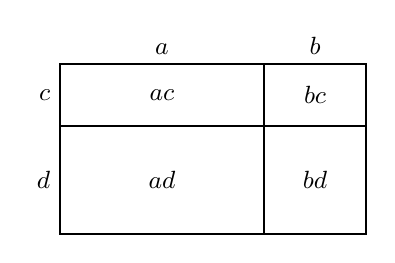
\begin{tikzpicture}[scale=0.72]
  \draw[thick] (0,0) rectangle (5.4,3.0);
  \draw[thick] (3.6,0) -- (3.6,3.0);
  \draw[thick] (0,1.9) -- (5.4,1.9);
  \node[font=\small] at (1.8,2.45) {$ac$};
  \node[font=\small] at (4.5,2.45) {$bc$};
  \node[font=\small] at (1.8,0.95) {$ad$};
  \node[font=\small] at (4.5,0.95) {$bd$};
  \node[above, font=\small] at (1.8,3.0) {$a$};
  \node[above, font=\small] at (4.5,3.0) {$b$};
  \node[left, font=\small] at (0,2.45) {$c$};
  \node[left, font=\small] at (0,0.95) {$d$};
\end{tikzpicture}

{\small Double distributivity as \omterm{def:g6:measure:area}{areas}: the rectangle
$(a+b) \times (c+d)$ splits into four smaller rectangles --- one per
term of the expansion.}
\end{omfigure}

\begin{method}[Expand and reduce]\label{met:g8:equations:reduce}
\begin{enumerate}
  \item Expand every \omterm{def:g2:mult:def}{product}, writing each term with its sign;
  \item collect like terms ($x^2$ with $x^2$, $x$ with $x$, numbers
        with numbers);
  \item check with a value: substitute e.g.\ $x = 2$ in the original
        and in the result --- equal outcomes catch most mistakes.
\end{enumerate}
\end{method}

\section{Solving equations}

\begin{definition}[Equation]\label{def:g8:equations:def}
An \emph{equation}\index{equation} is an equality with an unknown
number, written $x$ (or any letter). \emph{Solving} it means finding
all the values of $x$ making the equality true --- the
\emph{solutions}.
\end{definition}

\begin{theorem}[Balance rules]\label{thm:g8:equations:balance}
An \omterm{def:g8:equations:def}{equation} keeps exactly the same solutions when:
\begin{enumerate}
  \item the same number is added to (or subtracted from) both sides;
  \item both sides are multiplied (or divided) by the same
        \emph{nonzero} number.
\end{enumerate}
\end{theorem}
\admitted

\begin{omfigure}
\begin{tikzpicture}[scale=0.9]
  \draw[thick] (0,0) -- (0,0.5);
  \draw[thick] (-2.6,0.5) -- (2.6,0.5);
  \draw[thick] (-0.5,0) -- (0.5,0);
  \draw[thick] (-2.2,0.5) -- (-2.2,0.75);
  \draw[thick] (2.2,0.5) -- (2.2,0.75);
  \draw[omDef, fill=omDef!15] (-2.8,0.75) rectangle (-1.6,1.45);
  \node[font=\small] at (-2.2,1.1) {$x{+}3$};
  \draw[omThm, fill=omThm!15] (1.75,0.75) rectangle (2.65,1.45);
  \node[font=\small] at (2.2,1.1) {$8$};
  \node[below, font=\small] at (0,-0.25)
    {take $3$ away from both pans: $x = 5$};
\end{tikzpicture}

{\small An \omterm{def:g8:equations:def}{equation} is a balanced scale: whatever is done to one pan
must be done to the other, and the balance --- the equality ---
survives.}
\end{omfigure}

\begin{method}[Solving a first-degree equation]\label{met:g8:equations:solve}
\begin{enumerate}
  \item Expand and reduce each side if needed;
  \item add or subtract on both sides to gather the $x$-terms on one
        side, the plain numbers on the other;
  \item reduce, then divide both sides by the coefficient of $x$;
  \item \emph{check} by substituting the value found into the original
        \omterm{def:g8:equations:def}{equation}.
\end{enumerate}
\end{method}

\begin{example}\label{ex:g8:equations:solve}
Solve $7x - 5 = 4x + 16$:
\begin{align*}
7x - 5 &= 4x + 16 \\
7x - 4x &= 16 + 5
&& \text{(add $5$, subtract $4x$, on both sides)} \\
3x &= 21 \\
x &= 7 && \text{(divide both sides by 3).}
\end{align*}
Check: left side $7 \times 7 - 5 = 44$; right side
$4 \times 7 + 16 = 44$. The solution is $7$.
\end{example}

\begin{example}[With brackets and negatives]\label{ex:g8:equations:brackets}
Solve $3(x - 4) = 5 - 2(x + 1)$:
\begin{align*}
3x - 12 &= 5 - 2x - 2 && \text{(expand both sides)} \\
3x - 12 &= 3 - 2x && \text{(reduce)} \\
5x &= 15 && \text{(add $2x + 12$ to both sides)} \\
x &= 3 .
\end{align*}
Check: $3(3 - 4) = -3$ and $5 - 2(3+1) = 5 - 8 = -3$. \quad Solution:
$3$.
\end{example}

\begin{method}[Solving a problem with an equation]\label{met:g8:equations:problem}
\begin{enumerate}
  \item Choose the unknown: ``let $x$ be \dots'' (the quantity asked
        for, or a simpler related one);
  \item translate the story into an \omterm{def:g8:equations:def}{equation};
  \item solve it;
  \item interpret: answer the original question in a sentence, with
        units, and check the answer against the story.
\end{enumerate}
\end{method}

\begin{example}\label{ex:g8:equations:problem}
Lucas is $4$ years older than his sister; together their ages sum to
$26$. Let $x$ be the sister's age; then Lucas is $x + 4$, and
\[
x + (x + 4) = 26
\ \Longrightarrow\
2x + 4 = 26
\ \Longrightarrow\
2x = 22
\ \Longrightarrow\
x = 11 .
\]
The sister is $11$, Lucas is $15$. Check: $11 + 15 = 26$ and
$15 - 11 = 4$.
\end{example}

\section{Order and inequalities}

\begin{proposition}[Operations and order]\label{prop:g8:equations:order}
Adding the same number to both sides of an inequality preserves it;
multiplying both sides by a \emph{positive} number preserves it;
multiplying by a \emph{negative} number \emph{reverses} it:
\[
2 < 5 \ \text{ but }\ (-1) \times 2 > (-1) \times 5 .
\]
\end{proposition}
\admitted

\begin{example}\label{ex:g8:equations:inequality}
Solve $5 - 2x \leq 11$: subtract $5$ on both sides, $-2x \leq 6$;
divide by $-2$ \emph{and reverse}: $x \geq -3$. All the numbers
greater than or equal to $-3$ are solutions --- an \omterm{def:g8:equations:def}{equation} usually
has one solution, an inequality has a whole half-line of them.
\end{example}

\section{Exercises}

\begin{exercise}[$\star$]\label{exo:g8:equations:1}
Expand and reduce:
\[
5(2x + 3), \qquad
-3(4x - 1), \qquad
2(3x - 2) + 4(x + 5).
\]
\end{exercise}

\begin{exercise}[$\star$]\label{exo:g8:equations:2}
Expand and reduce:
\[
(x + 2)(x + 7), \qquad
(3x + 1)(2x - 5), \qquad
(x - 4)(x - 6).
\]
\end{exercise}

\begin{exercise}[$\star$]\label{exo:g8:equations:3}
Is $x = 3$ a solution of $4x - 5 = 7$? Of $2x + 1 = x + 4$? Of
$x^2 = 6x - 9$? (Substitute and compare both sides.)
\end{exercise}

\begin{exercise}[$\star$]\label{exo:g8:equations:4}
Solve, with a check:
\[
x + 9 = 4, \qquad
5x = -35, \qquad
\frac{x}{3} = 8, \qquad
2x - 7 = 13 .
\]
\end{exercise}

\begin{exercise}[$\star$]\label{exo:g8:equations:5}
Solve:
\[
6x + 5 = 2x + 25, \qquad
9 - 4x = x - 11, \qquad
3(x + 2) = 2x + 11 .
\]
\end{exercise}

\begin{exercise}[$\star$]\label{exo:g8:equations:6}
Solve $4(2x - 3) = 5(x + 6)$, expanding first, and check your
solution.
\end{exercise}

\begin{exercise}[$\star$]\label{exo:g8:equations:7}
Translate and solve: ``three times a number, decreased by $8$, equals
$19$''; ``the double of a number increased by $5$ equals the number
increased by $12$''.
\end{exercise}

\begin{exercise}[$\star\star$]\label{exo:g8:equations:8}
A rectangle's length is $5$ cm more than its width, and its \omterm{def:g6:measure:perimeter}{perimeter}
is $58$ cm. Let $x$ be the width: write an \omterm{def:g8:equations:def}{equation}, solve it and give
the two dimensions.
\end{exercise}

\begin{exercise}[$\star\star$]\label{exo:g8:equations:9}
Three consecutive whole numbers have \omterm{def:g1:addition:def}{sum} $141$. Call the middle one
$n$ and find all three.
\end{exercise}

\begin{exercise}[$\star\star$]\label{exo:g8:equations:10}
Solve the inequalities and describe the solutions:
\[
3x + 4 > 19, \qquad
7 - 2x \geq 1, \qquad
5(x - 1) < 2x + 7 .
\]
\end{exercise}

\begin{exercise}[$\star\star$]\label{exo:g8:equations:11}
Mia has $140$ euros in savings and adds $15$ euros each month; Tom
has $200$ euros and adds $10$ euros each month. After how many months
will Mia have strictly more than Tom? (Set up an inequality.)
\end{exercise}

\begin{exercise}[$\star\star\star$]\label{exo:g8:equations:12}
Solve the \omterm{def:g8:equations:def}{equation} $\dfrac{x + 3}{4} = \dfrac{2x - 1}{5}$.
(Multiply both sides by $20$, the common \omterm{def:g4:fractions:def}{denominator}, then proceed as
usual; check your solution in the original \omterm{def:g8:equations:def}{equation}.)
\end{exercise}

\section{Problem: Remarkable identities and the staircase of odd
numbers}

\begin{problem}[{Weekend problem --- $(a+b)^2$, $(a-b)^2$,
$(a+b)(a-b)$, and the sum $1 + 3 + 5 + \dots + (2n-1) = n^2$}]
\label{pb:g8:equations:1}
Three expansions come up so often that algebra knows them by
heart: they are called the \emph{remarkable identities}. This
problem derives them from double distributivity
(\cref{thm:g8:equations:expand}), turns them into a mental-arithmetic
superpower, uses them to prove a beautiful fact about \omterm{def:g3:numbers:evenodd}{odd numbers},
and ends by solving \omterm{def:g8:equations:def}{equations} of a brand-new kind: \omterm{def:g8:equations:def}{equations} with a
square in them.

\medskip
\noindent\textbf{Part I --- The three identities.}
\begin{enumerate}
  \item Expand $(a + b)^2 = (a + b)(a + b)$ and reduce, to prove
        \[
        (a + b)^2 = a^2 + 2ab + b^2 .
        \]
  \item Prove likewise the two companions:
        \[
        (a - b)^2 = a^2 - 2ab + b^2,
        \qquad
        (a + b)(a - b) = a^2 - b^2 .
        \]
  \item Draw a square of side $a + b$, split each side into $a$
        and $b$, and cut the square into four pieces. Which piece
        of the first identity does each part of the picture
        represent?
  \item Mental arithmetic: use the identities to compute, without
        posing any multiplication,
        \[
        101^2, \qquad 99^2, \qquad 49 \times 51 .
        \]
  \item A classic trap: Zoe writes ``$(a + b)^2 = a^2 + b^2$''.
        Test her formula with $a = 3$, $b = 4$, and explain on the
        picture of question 3 exactly which pieces her formula
        forgets.
\end{enumerate}

\medskip
\noindent\textbf{Part II --- The staircase of \omterm{def:g3:numbers:evenodd}{odd numbers}.}
\begin{enumerate}[resume]
  \item Compute $1$, then $1 + 3$, then $1 + 3 + 5$, then
        $1 + 3 + 5 + 7$, then $1 + 3 + 5 + 7 + 9$. What do you
        notice about the results?
  \item Explain why the $n$-th \omterm{def:g3:numbers:evenodd}{odd number} is $2n - 1$ (check:
        $n = 1, 2, 3$ give $1, 3, 5$).
  \item Use an identity of Part I to expand and reduce
        $(n + 1)^2 - n^2$. What does the result have to do with
        question 7?
  \item Question 8 says: to pass from a square of side $n$ to a
        square of side $n + 1$, one adds exactly the next \omterm{def:g3:numbers:evenodd}{odd
        number} of unit cells --- an L-shaped border along two
        sides and the corner. Starting from $1 = 1^2$ and growing
        the square one layer at a time, explain why
        \[
        1 + 3 + 5 + \dots + (2n - 1) = n^2 :
        \]
        the \omterm{def:g1:addition:def}{sum} of the first $n$ \omterm{def:g3:numbers:evenodd}{odd numbers} is the $n$-th square.
  \item Deduce, without adding them up one by one: the value of
        $1 + 3 + 5 + \dots + 99$; and how many \omterm{def:g3:numbers:evenodd}{odd numbers}, starting
        from $1$, add up to exactly $400$.
\end{enumerate}

\medskip
\noindent\textbf{Part III --- \omterm{def:g8:equations:def}{Equations} with a square.}
\begin{enumerate}[resume]
  \item Recognize a remarkable identity in $x^2 + 6x + 9$, and
        solve the \omterm{def:g8:equations:def}{equation} $x^2 + 6x + 9 = 0$.
  \item Explain, using the sign-and-distance rule of
        \cref{thm:g8:negprod:rules}, why a \omterm{def:g2:mult:def}{product} of two numbers
        can be \omterm{def:g1:counting:zero}{zero} \emph{only if} one of the two factors is \omterm{def:g1:counting:zero}{zero}.
        Use this to solve $(x - 2)(x + 5) = 0$.
  \item Solve $x^2 = 49$ by moving everything to one side and
        factoring $x^2 - 49$ with the third identity. How many
        solutions does this \omterm{def:g8:equations:def}{equation} have --- and how does that
        differ from every \omterm{def:g8:equations:def}{equation} solved in this chapter so far?
  \item In \cref{exo:g8:equations:3} you checked that $x = 3$ is
        a solution of $x^2 = 6x - 9$. Show that it is the
        \emph{only} one: bring everything to one side, recognize
        an identity, and conclude.
  \item Finale: compute $2026^2 - 2025^2$ in your head, and
        explain with an identity why the \omterm{ex:g1:subtraction:difference}{difference} of two
        consecutive squares is always the \omterm{def:g1:addition:def}{sum} of the two numbers
        --- which is question 8 all over again.
\end{enumerate}
\end{problem}
